\chapter{Experimental Setup}\label{chapter:second_real_chapter}

\section{Implementation details}
\subsection{Dataset}
\paragraph{COCO\cite{lin2015microsoftcococommonobjects}} is a publicly available dataset and has a multitude of labels. The semantic mask are extrated from the 2017 Panoptic annotations. This set contains more then 100k images that are densly annotated with both the semantic class and instance. There are a total of 133 different classes which belong to 27 'supercategories'. To reduce the complexity and speed up convergence, only the supercategories are used. The images are scaled to 128x128 to allow for a bigger batch-size.

\paragraph{NOTE: Not yet sure if I will use this. CamVid\cite{BrostowFC:PRL2008,BrostowSFC:ECCV08}} is a high quality video database of driving data. It contains 702 frames with a resolution of 960x720, which are semantically labeled with 32 classes. It is often used as benchmark in real-time semantic segmentation tasks.


\subsection{Training Settings}
All models are implemented in PyTorch \cite{Ansel_PyTorch_2_Faster_2024} using an adapted version of the segmentation models repository \cite{Iakubovskii:2019}. All code and configs required to train the models and reproduce the experiments can be found on github \footnote[1]{\url{https://github.com/Generative-AI-TUe/msc-project-1297333}}. All models are trained on the NVIDIA Geforce RTX 2080 TI. The gradients are clipped using the norm, with a max value of 10. The AdaMax\cite{kingma2017adammethodstochasticoptimization} is used with a cosine annealing learning rate. Each model is trained on 20.000 minibatches.

\section{Comparison against the baseline models}
We compare our method against the two baseline methods, UNet and FPN. Each method is trained from scratch and using a pretrained encoder on ImageNet \cite{deng2009imagenet}. The mIoU is reported, aswell as the FLOPs and inference speed on the NVIDIA RTX 1070. 
TODO Add the results here. I am not yet finished with the ablation study to determine the best model setup. I will try to keep the UNet and FPN settings as close as possible to the VAE settings.

These experiments are not yet fully done, however here are some preliminary results from the pretrained VAE. The Loss values and Jaccard Index (JI) can be seen in Table \ref{tab:seg-vae}. The preliminary results seem to indicate that the model is overfitting quickly if the 

\begin{table}[!ht]
    \centering
    \caption{Various metrics for the segmentation value for the pretrained, frozen VAE, after only 1000 optimization steps}
    \label{tab:seg-vae}
    \begin{tabular}{ccccc}
        \hline
        Model Variant & Kl-Divergence & CrossLoss (x1e6) & Eval JI & Train JI \\
        \hline
        pre-b0.01     & 80200         & 0.8              & 0.092   & 0.129    \\
        pre-b0.1      & 31250         & 0.8              & 0.154   & 0.129    \\
        pre-b1        & 8190          & 0.8              & 0.090   & 0.120    \\
        pre-b10       & 2089          & 0.8              & 0.108   & 0.124    \\
        Seg-Var       & n.a           & n.a              & n.a     & n.a      \\
        UNET          & n.a           & 1.3              & 0.140   & 0.137    \\
        \hline
    \end{tabular}
\end{table}


\section{Ablation Study}
\subsection{Influence of the backbone}
We first analyze the influence of the backbone on the performance of the VAE task by comparing the following backbones, MobilenetV2 \cite{sandler2019mobilenetv2invertedresidualslinear}, EfficientNet \cite{tan2020efficientnetrethinkingmodelscaling} and Resnet50 \cite{he2015deep}. The results of the 

\subsection{Influence of the Beta factor}
We also analyze the effect of the beta factor on the quality of the encoder features. This is done by pre-training models with varying values for beta, after which they are finetuned for the segmentation task. The results can be seen in Table \ref{tab:beta-vae-loss-values}. Some examples of the reconstruction capabillities can be seen in Figure \ref{fig:beta-vae-recon-examples}.

\begin{table}[!ht]
    \centering
    \caption{Loss values resulting from training a Beta-VAE for various $\beta$ values}
    \label{tab:beta-vae-loss-values}
    \begin{tabular}{ccc}
        \hline
        $\beta$ & Kl-Divergence & Reconstruction Error (x1e5) \\
        \hline
        0.01    & 80200         & 1.9                         \\
        0.1     & 31250         & 1.5                         \\
        1       & 8190          & 2.7                         \\
        10      & 2089          & 2.2                         \\
        100     & (node crashed & mid run)                    \\
        \hline
    \end{tabular}
\end{table}

\begin{figure}[!ht]
    \centering
    \caption{Example reconstructions for $\beta$-vae.}
    \label{fig:beta-vae-recon-examples}
    \subfloat[Original, $\beta$ = 0.01]{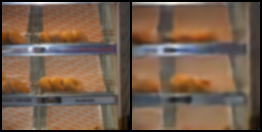
\includegraphics[width=0.45\linewidth]{figures/beta-vae/b0.01-0.png}}
    \subfloat[Original, $\beta$ = 0.1]{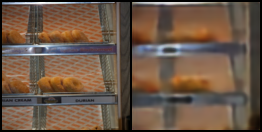
\includegraphics[width=0.45\linewidth]{figures/beta-vae/b0.1-0.png}} \quad
    \subfloat[Original, $\beta$ = 1]{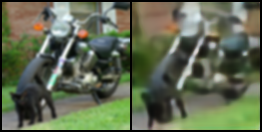
\includegraphics[width=0.45\linewidth]{figures/beta-vae/b1-0.png}}
    \subfloat[Original, $\beta$ = 10]{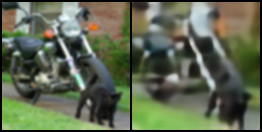
\includegraphics[width=0.45\linewidth]{figures/beta-vae/b10-0.png}}
\end{figure}



\subsection{Unfreezing}
To show the impact of freezing the encoder, we finetune a model that does not change the encoder model and compare it to one that is not frozen. The benefit of freezing the encoder is that the original $p(z |x)$ is preserved which can be used for anomaly detection. Furthermore, it makes the switch to an multimodal VAE, such as proposed in \cite{vasco2020mhvae}, possible.

\subsection{Skip Connection}
To understand the importance of the skip connections which are added after the pretraining. We will show the effect of this by incrementally removing more skip connections.

\subsection{Probabilistic Inference}
TODO not entirely sure if I have enough time for this
Another potential benefit of the VAEseg is the probabilistic nature of the model. Using bootstrapping, an uncertainty measure can be created. To understand if this certainty measure is a useful predictor of the actual certainty of the output. The ECE is reported for various sizes of bootstrapping.

\section{Understanding potential benefits of VAE}
\subsection*{ImageNet Bias}
\#TODO provide some examples of the (racial) bias problems of Imagenet. Might be able to generalize it to human made labels, hence benefit of VAE.

As previous research already has shown (TODO link research), models that use a pretrained backbone which is trained on the ImageNet dataset, contain various biases. As our backbone is not trained on ImageNet a small qualitative research will be done on the 2 models. To detect wheter the bias differs between the VASegm and an UNet-segmentation model. This is done by training two models, one using a frozen encoder which is trained on ImageNet, and one that is trained using the VAE. Based on some initial datavisualization it was suggested that ImageNet contained some racial biases in which it depicted persons of color more often as animals in comparison to the wrongly predicted caucasians people.


% \subsection*{General Metrics}
% For all of the above experiments the following metrics will be tracked to get insight in the quality of the model.

% \begin{table}[]
%     \begin{tabular}{l|l|l}
%         Metric                      & Formula                                   & Reason                                     \\
%         \hline
%         Precision                   & $\frac{TP}{TP + FP}$                      & Standard practice                          \\
%         Recall                      & $\frac{TP}{TP + FN}$                      & Standard practice                          \\
%         Segmentation quality        & $\frac{\|TP\|}{\|FP\| + \|TP\| + \|FN\|}$ & Quantifly compare accuracy of the model    \\
%         Expected Callibration Error &                                           & Check uncertainty prediction is reliable.
%     \end{tabular}
% \end{table}

% \footnote[1]{ECE is taken from \cite{guo2017calibration}}
